\documentclass[10pt,a4paper]{scrartcl}
\usepackage[utf8x]{inputenc}
\usepackage{ngerman}
\usepackage{amsmath}
\usepackage{amsfonts}
\usepackage{amssymb}
\usepackage{makeidx}
\usepackage{graphicx}
\usepackage{bytefield2}
\usepackage{marginnote}
\usepackage[left=2cm,right=2cm,top=2cm,bottom=2cm]{geometry}
\author{Sven Schröder, Jens Bork}
\title{Dokumentation -- NXT}
\begin{document}
\maketitle
\tableofcontents
\section{Entwurf}
\subsection{Software}
Beim Entwurf der Software für unseren Teil der Aufgabe hatten wir zwei Dinge zu beachten, die eingeschränkte Rechenleistung\footnote{8-Bit ARM mit 48 MHz Takt, 64KB RAM} des LEGO$^\copyright$ Mindstorms$^\copyright$ NXT Brick (im folgenden nur noch Brick genannt) und die durch LEGO$^\copyright$ begrenzte Anzahl von Robotern auf maximal 4. 
\subsubsection{nxc -- Not eXactly C}
nxc ist die für LEGO$^\copyright$ NXT native Programmiersprache mit einem Compiler, welche für diversen Plattformen erhältlich ist. Obwohl die Syntax von nxc der Programmiersprache C ähnlich ist, ist sie in ihrem Umfang erheblich eingeschränkt. Aus dem Fehlen des Pointerkonzept resultiert unter anderem der Verlust auf die Speicherverwaltung direkt einwirken zu können.
\subsubsection{nxt-python-framework}
Das nxt-python-framework\footnote{http://code.google.com/p/nxt-python/} agiert als Interface, welches die von LEGO$^\copyright$ in dem "`Bluetooth Development Kit"' veröffentlichten direkten Kommandos, nutzt um mit der Hardware zu interagieren.\\
\\
Wie wird dies erreicht?\\
Mit LEGO$^\copyright$ NXT ist es möglich, dass sich bei maximal vier NXTs einer zum Master erklärt. Der Master kann nun durch speziell kodierte Befehle die anderen drei NXTs fernsteuern. Dieses Verhalt macht sich das nxt-python-framework zu nutze und täuscht maximal 3 NXTs vor, dass es ein NXT-Master sei. Wenn dies geschehen ist können die NXTs von PC-Seite ferngesteuert werden.\\
\\
Vorteil: Durch die Nutzung von nxt-python integriert sich die Komponente NXT-Erkunder nahtlos in das übrige System.\\
\\
Nachteil: Der synchrone Start bzw. Stopp von zwei Motoren ist nur schwerlich realisierbar, da zwei Befehle benötigt würden, die nacheinander verschickt und auf NXT-Seite nacheinander ausgewertet werden würden. \\
\\
Wegen dem immensen Vorteil der einfachen Integration in das Restsystem und dem Nachteil der asynchronen Ansteuerung von Motoren entstand die Idee die beiden Programmiersprachen (nxc und python) zu kombinieren.
\subsubsection{hybrider Ansatz}
Die Kombination von nxc und nxt-python wurde wie folgt realisiert. Es wurde in einfaches Kommunikationsprotokoll (siehe Abbildung \ref{protokoll} auf Seite \pageref{protokoll}) konzipiert durch welches der Aufruf von in nxc implementierten Funktionen durch nxt-python ermöglicht wird.

\subsection{Idee 1 $\rightarrow$ Modell 1}%Kettenfahrzeug + Radar
\subsubsection{Idee}
Unsere erste Idee bestand im Prinzip aus zwei unabhängigen Ideen. Zum Einen wollten wir ein Fahrgestell konzipieren, das auch bei unwegsamen Gelände eine kontrollierte Bewegung des Explorer ermöglichen würde und zum Anderen wollten wir einen Sensor der schon viele Informationen über die Umgebung sammelt ohne, dass der Explorer jeden Quadratzentimeter abfahren muss.
\subsubsection{Konstruktion}
Die Konstruktion bestand aus einem kettengetriebenen Fahrzeug, welches mit Hilfe eines Radars seine Umgebung wahrnahm (siehe Abbildung \ref{modell1} auf Seite \pageref{modell1}). Die Ketten waren dabei fest gespannt um mögliches schlüpfen der Kette über die Achse zu vermeiden und so eine Ungenauigkeit bei der Fahrt zu vermeiden. Des Weiteren bestanden sie aus Gummi und hatten eine große Auflagefläche zum Boden und somit eine möglichst hohe Reibung zum Boden. Der Radar bestand aus einem Motor der über einige Zahnräder und einer Schnecke einen Ultraschallsensor bewegte.\\
Verbaute Sensoren und Motoren:
\begin{itemize}
\item zwei Motoren für den Antrieb
\item ein Motor für den Radar
\item ein Kompass-Sensor zur Ermittlung der Ausrichtung des Fahrzeuges
\item ein Lichtstärke-Sensor zur Zielfindung
\end{itemize}
\begin{figure}[ht]
	\centering
  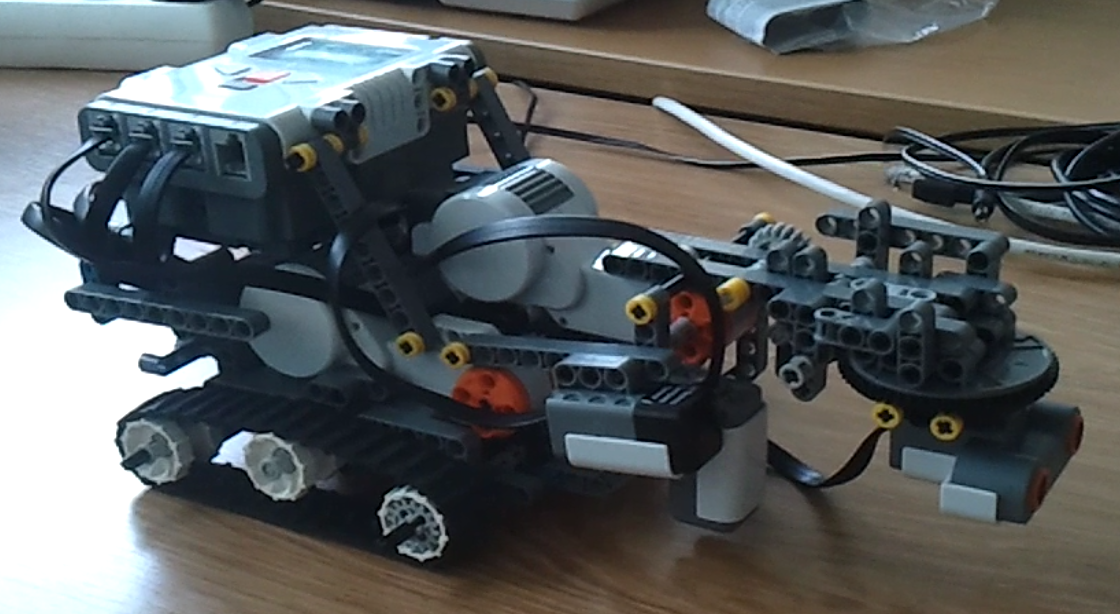
\includegraphics[width=0.9\textwidth, angle=0]{modell1.png}
	\caption{Modell 1}
	\label{modell1}
\end{figure}
\subsubsection{Test}
Getestet haben wir sowohl das Fahrverhalten des Kettenfahrzeuges als auch die Möglichkeit mit dem Radar die Umgebung wahrzunehmen. Hierbei wurde besonders Wert darauf gelegt die Abweichung zum Ist-Wert zu ermitteln.\\
Beim Fahrzeug war es wichtig herauszufinden ob es geradeaus fahren kann und ja mit welcher Abweichung auf verschieden Distanzen (20cm, 50cm, 1m) zu rechnen war. Des Weiteren musste ermittelt werden ob das Fahrzeug in der Lage war sich auf der Stelle zu drehen und dies möglichst genau nach der Vorgabe eines vorher angegeben Winkels. Hierfür wurden mehrere Test mit verschiedensten Winkeln durchgeführt bei denen das Fahrzeug sich so oft drehen musste bis es wieder auf seine Ausgangsposition angelangt ist z.B. vier mal eine Drehung um 90° im Uhrzeigersinn.
Der Radar wurde auf seine Genauigkeit getestet, als auch auf sein Verhalten bei verschiedenen Materialien und Winkel zu den verschiedenen Objekten.
\subsubsection{Pros \& Cons}
Pros:
\begin{itemize}
\item geringe Abweichung bei der Fahrt durch die hohe Reibung der Gummiketten
\item hohe Geländetauglichkeit durch Kettenantrieb
\item kennt das Gebiet vor sich und kann vorausschauend fahren
\end{itemize}
Cons:
\begin{itemize}
\item hohe Abweichung beim drehen
\item sehr hohe Abweichung des Ultraschallsensors wenn nicht im 90° zum Hindernis
\item hohe Ungenauigkeit beim drehen des Radarkopfes durch das Getriebe
\end{itemize}
\subsubsection{Fazit}
Die Idee ist alles in allem nicht schlecht aber die Umsetzung mittels LEGO$^\copyright$ ist nicht praktikabel. Die hohen Ungenauigkeiten und die komplett Aussetzer des Ultraschallsensors lassen uns keine andere Wahl als eine neues Fahrzeug zu entwerfen. Hierbei muss sowohl der Antrieb als auch die Sensorkonstruktion überdacht werden. An einen Einsatz dieses Models ist nicht zu denken.
\subsection{Idee 2 $\rightarrow$ Modell 2}%angepasstes Grundmodell + riesiger Stoßdämpfer
\subsubsection{Idee}
Da wir bei unserer ersten Idee feststellen mussten das ein kettengetriebenes Fahrzeug zu hohe Ungenauigkeiten verursachte, musste hier eine Alternative gefunden werden, welche aber keine Einschränkungen bei der Bewegungsfreiheit des Fahrzeuges macht d.h. möglichst genaues (vorwärts/rückwärts) Fahren und auf der Stelle wenden können.\\
Auch eine Alternative für den Radar musste her. Hierbei wurde in Kooperation mit dem MCC-Team vereinbart das nicht Hindernisse gefunden werden, sondern davon ausgegangen wird das die gefahren Strecke des Explores frei ist, sozusagen wurde das Bild der Karte invertiert. Dies ermöglichte uns nur auf Hindernisse reagieren zu müssen und nicht wie vorher Informationen über den Bereiche des Einsatzgebietes zu sammeln.
\subsubsection{Konstruktion}
Unsere Konstruktion 2 (siehe Abbildung \ref{modell2} auf Seite \pageref{modell2}) erhielt nun ein 2-Achsen Antrieb, welcher es uns ermöglichte durch gleichzeitiges ansteuern der Motoren gerade Strecken zu fahren, als auch durch entgegengesetztes ansteuern sich auf der Stelle zu drehen. Als Zusatz wurde noch ein Omni-Wheel verbaut, welches dem Gefährt mehr Stabilität verleihen sollte. Um auf Hindernisse reagieren zu können, wurden an der Vorderseite des Fahrzeuges drei Touchsensoren befestigt. Diese sollten auslösen sobald das Fahrzeug vor ein Hindernis fuhr.\\
Verbaute Sensoren und Motoren:
\begin{itemize}
\item zwei Motoren für den Antrieb
\item drei Touch-Sensoren um Hindernisse zu finden
\item ein Lichtstärke-Sensor zur Zielfindung
\end{itemize}
\begin{figure}[ht]
	\centering
  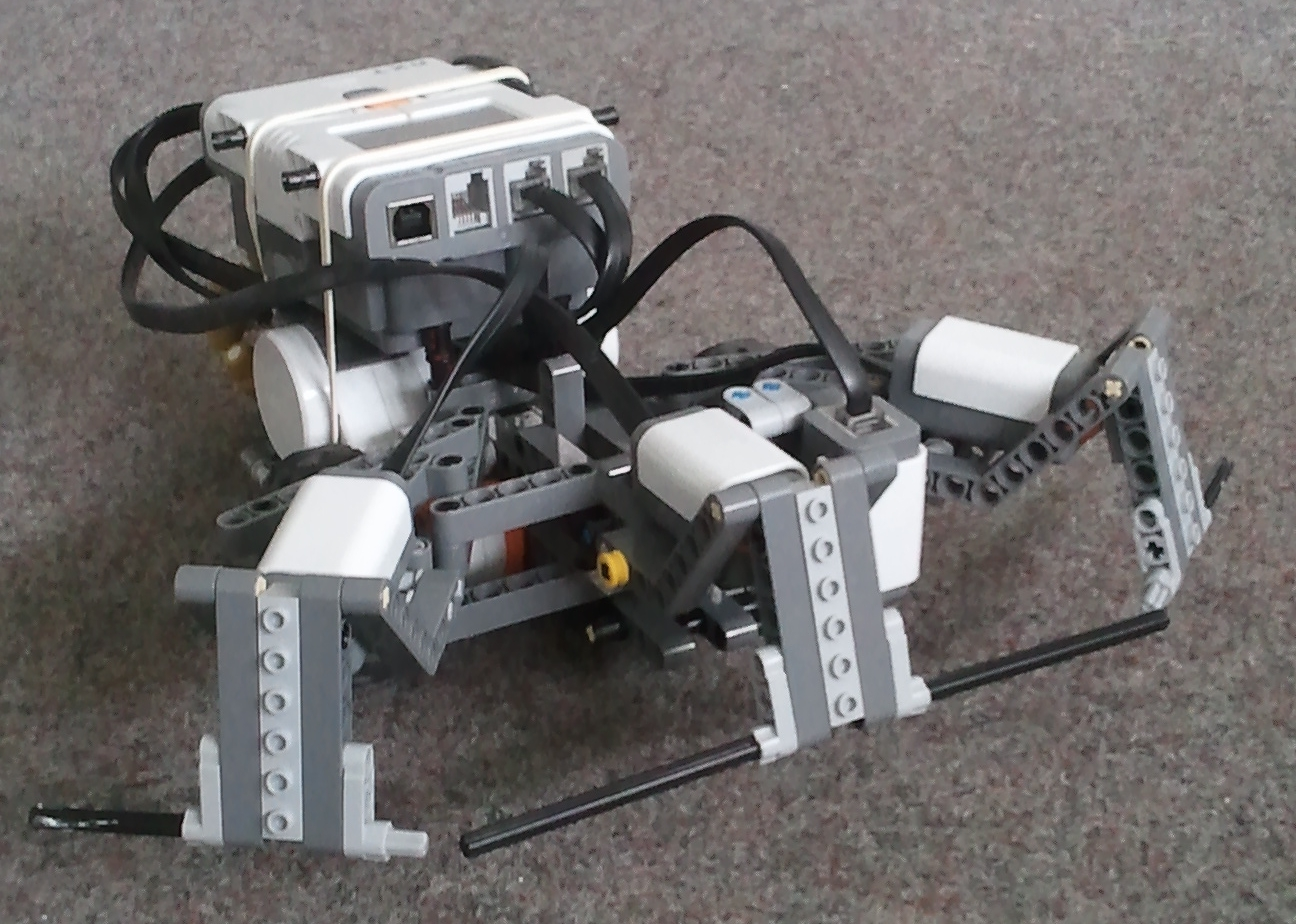
\includegraphics[width=0.9\textwidth, angle=0]{modell2.jpg}
	\caption{Modell 2}
	\label{modell2}
\end{figure}
\subsubsection{Test}
Auch beim zweiten Model wurden die oben schon beschrieben Tests für den Antrieb durchgeführt. Die Sensoren wurden in ihrer Anordnung getestet um eine möglichst optimale Anordnung zu finden. 
\subsubsection{Pros \& Cons}
Pros:
\begin{itemize}
\item geringe Abweichung beim fahren
\item geringe Abweichung beim drehen
\item hohe Aussagekraft bzgl. Sensorevents da nur Touch-Sensoren verbaut wurden
\end{itemize}
Cons:
\begin{itemize}
\item keine Aussagen über das Gebiet vor dem Fahrzeug möglich
\item Fahrzeug kann nur noch reagieren und kaum intelligent handeln
\item Verhaken der Touch-Sensorkonstruktion
\end{itemize}
\subsubsection{Fazit}
Bei der zweiten Konstruktion überzeugt das Antriebsmodel durch seine geringen Abweichungen und seine Agilität. Die Sensoranordnung hingegen lässt noch einige Wünsche offen. Die fehlende Voraussicht ist dabei das größte Manko. An einen Einsatz dieses Model ist ebenfalls nicht zu denken. Eine Verbesserung des Sensorkonstrukts ist nötig.
\subsection{Idee 3 $\rightarrow$ Modell 3}%angepasstes Grundmodell + verbesserte Stoßdämpfer
\subsubsection{Idee}
Das in Idee 2 entwickelte Antriebsmodel hat uns überzeugt. Im dritten Anlauf wird sollte nur noch die Sensoranordnung überdacht werden. Dem Bereich vor dem Fahrzeug sollte dabei mehr Beachtung geschenkt werden, um bessere und intelligentere Entscheidungen treffen zu können.
\subsubsection{Konstruktion}
Bei der dritten Konstruktion (siehe Abbildung \ref{modell3} auf Seite \pageref{modell3}) wurde das Antriebsmodel der zweiten Konstruktion übernommen. Bei den Sensoren wurde der mittlere Touch-Sensor durch ein Ultraschall-Sensor ersetzt. Dieser ermöglichte es die freie Strecke vor dem Fahrzeug zu ermitteln.\\
Verbaute Sensoren und Motoren:
\begin{itemize}
\item zwei Motoren für den Antrieb
\item zwei Touch-Sensoren um Hindernisse zu finden
\item ein Ultraschall-Sensor um den Bereich vor dem Fahrzeug zu überblicken.
\item ein Lichtstärke-Sensor zur Zielfindung
\end{itemize}
\begin{figure}[ht]
	\centering
  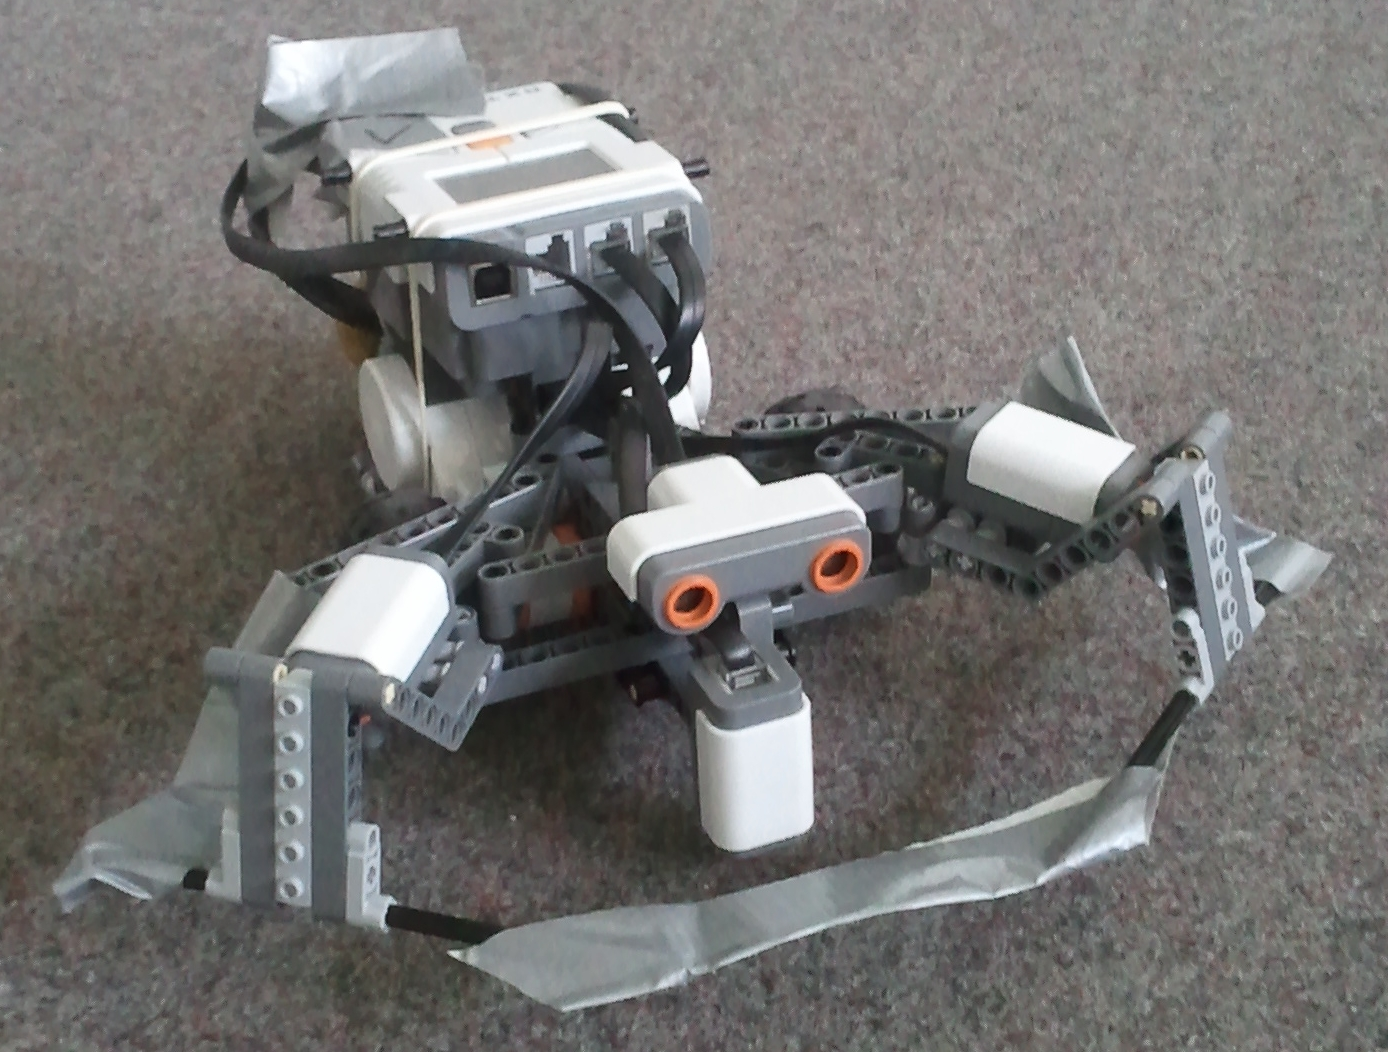
\includegraphics[width=0.9\textwidth, angle=0]{modell3.jpg}
	\caption{Modell 3}
	\label{modell3}
\end{figure}
\subsubsection{Test}
Auch beim dritten Model wurden alle Antriebstests durchgeführt. Die neue Sensoranordnung wurde mit mehreren Testaufbauten auf ihre Einsatztauglichkeit geprüft. Hierbei wurden mögliche Anordnungen von Hindernissen konstruiert und die Sensorevents ausgewertet.
\subsubsection{Pros \& Cons}
Pros:
\begin{itemize}
\item geringe Abweichung beim fahren
\item geringe Abweichung beim drehen
\item freie Strecke vorm Fahrzeug bekannt
\end{itemize}
Cons:
\begin{itemize}
\item Verhaken der Touch-Sensorkonstruktion
\end{itemize}
\subsubsection{Fazit}
Das dritte Model überzeugt durch seinen Antriebsmodel, sowie durch die verbesserte Sensoranordnung gegenüber des zweiten Models. Aber auch dieses Model ist mit Vorsicht zu benutzen. Die Möglichkeiten des Verhaken der Fahrzeuge ist ein großes Problem das es noch zu beseitigen gibt. An einen Einsatz ist nur bedingt zu denken.
\subsection{Fazit und Entscheidung}
Das erste Model ist für raues Gelände bestens geeignet. Durch seine hohen Abweichungen beim Fahren und des nicht zuverlässigen Ultraschall-Sensors im Radar aber kein Kandidat für die Lösung unseres Problems.\\
Das zweite Model überzeugt durch seine Genauigkeit beim Fahren und auch die Aussagekraft der Sensoranordnung. Allerdings fehlt uns hier das gewisse etwas um ein möglichst elegante Lösung für die autonome Erkundung eines Gebietes.\\
Von allen Model schneidet das dritte am besten ab. Es erbt die guten Fahrteigenschaften des zweiten Models und biete uns dazu noch die Möglichkeit durch seine überarbeitete Sensoranordnung möglichst intelligent das Problem zu lösen. 
\section{Kommunikation}
\subsection{Bluetooth}
\subsection{Kommunikationsprotokoll PC $\leftrightarrow$ NXT}
anfänglich 3-way-handshake wegen missverständnis
\begin{figure}[h]
Kommunikation PC $\rightarrow$ NXT:$\qquad$
\begin{bytefield}[bitwidth=2em]{7}
\bitheader{0-6} \\
\bitbox{1}{A} & \bitbox{1}{;} & \bitbox{1}{ID} & \bitbox{1}{;} & \bitbox{1}{F} & \bitbox{1}{,} & \bitbox{1}{W}
\end{bytefield}\\
~\\
Kommunikation PC $\leftarrow$ NXT:$\qquad$
\begin{bytefield}[bitwidth=2em]{9}
\bitheader{0-8} \\
\bitbox{1}{A} & \bitbox{1}{;} & \bitbox{1}{ID} & \bitbox{1}{;} & \bitbox{1}{T} & \bitbox{1}{,} & \bitbox{1}{W} & \bitbox{1}{,$_2$} & \bitbox{1}{W$_2$}
\end{bytefield}
\\
\\
\texttt{\underline{Legende:}\\ A = Typ der Nachricht (m = Nachricht, r = m erhalten, a = r erhalten)\\ F = Funktion die aufgerufen werden soll\\ W = Zahlwert \\ T = Typ der Antwort\\ $_2$ = optional}

\caption{Kommunikationsprotokoll 3-way-handshake}\label{protokoll_alt}
\end{figure}
\\
\begin{figure}[h]
Kommunikation PC $\rightarrow$ NXT:$\qquad$
\begin{bytefield}[bitwidth=2em]{5}
\bitheader{0-4} \\
\bitbox{1}{ID} & \bitbox{1}{;} & \bitbox{1}{F} & \bitbox{1}{,} & \bitbox{1}{W}
\end{bytefield}\\
~\\
Kommunikation PC $\leftarrow$ NXT:$\qquad$
\begin{bytefield}[bitwidth=2em]{7}
\bitheader{0-6} \\
\bitbox{1}{ID} & \bitbox{1}{;} & \bitbox{1}{T} & \bitbox{1}{,} & \bitbox{1}{W} & \bitbox{1}{,$_2$} & \bitbox{1}{W$_2$}
\end{bytefield}
\\
\\
\texttt{\underline{Legende:}\\ F = Funktion die aufgerufen werden soll\\ W = Zahlwert \\ T = Typ der Antwort\\ $_2$ = optional}

\caption{Kommunikationsprotokoll}\label{protokoll}
\end{figure}
\subsection{Kommunikation mit dem MCC}
\section{Logik}
Problem das der Robo blockiert, das Programm aber nicht
\subsection{Explorationsalgorithmen}
In der Welt der autonomen Rasenmäh- und Staubsaugroboter haben sich vier Algorithmen durchgesetzt:
\begin{enumerate}
\item Touch and Go\footnote{hier simple genannt}
\item circle
\item radar
\item Wandverfolgung
\end{enumerate}
1 -- 3 werden im Folgenden näher besprochen. 4 konnte aufgrund der begrenzten Anzahl an Sensoren nicht implementiert werden und bleibt deshalb außen vor. 
\subsubsection{Exploration -- simple}
\subsubsection{Exploration -- circle}
\subsubsection{Exploration -- radar}
\subsection{GoToPoint}
\end{document}
